\usetikzlibrary{positioning, chains, shapes.geometric, fit, shapes, arrows.meta, calc, backgrounds}

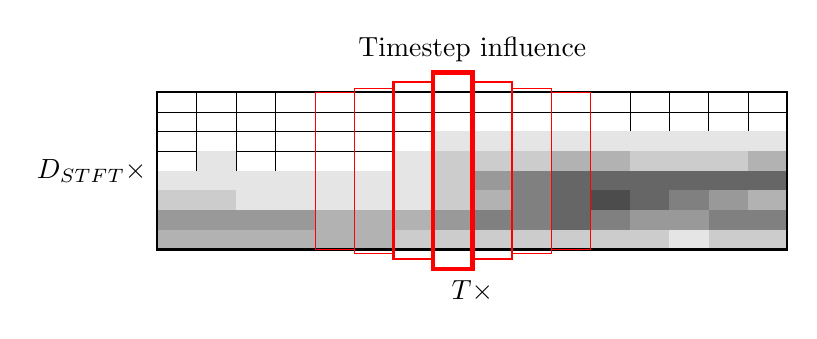
\begin{tikzpicture}[
    very thick,
    arrow/.style={
        -latex,
        very thick,
        rounded corners=0.2cm
    },
    ]

% ------ Grid ------

\draw[transform canvas={xscale=2}, step=0.25cm, ultra thin] (-2, 1) grid (2, 3);
\node[anchor=south] at (0, 3.25) {Timestep influence};
\node[anchor=east] at (-4, 2) {$D_\text{STFT}\times$};
\node[anchor=north] at (0, 0.75) {$T\times$};

% ------ Values ------

\fill[black!30] (-4.0, 1.0) rectangle (-3.5, 1.25);
\fill[black!30] (-3.5, 1.0) rectangle (-3.0, 1.25);
\fill[black!30] (-3.0, 1.0) rectangle (-2.5, 1.25);
\fill[black!30] (-2.5, 1.0) rectangle (-2.0, 1.25);
\fill[black!30] (-2.0, 1.0) rectangle (-1.5, 1.25);
\fill[black!30] (-1.5, 1.0) rectangle (-1.0, 1.25);
\fill[black!20] (-1.0, 1.0) rectangle (-0.5, 1.25);
\fill[black!20] (-0.5, 1.0) rectangle (0.0, 1.25);
\fill[black!20] (0.0, 1.0) rectangle (0.5, 1.25);
\fill[black!20] (0.5, 1.0) rectangle (1.0, 1.25);
\fill[black!20] (1.0, 1.0) rectangle (1.5, 1.25);
\fill[black!20] (1.5, 1.0) rectangle (2.0, 1.25);
\fill[black!20] (2.0, 1.0) rectangle (2.5, 1.25);
\fill[black!10] (2.5, 1.0) rectangle (3.0, 1.25);
\fill[black!20] (3.0, 1.0) rectangle (3.5, 1.25);
\fill[black!20] (3.5, 1.0) rectangle (4.0, 1.25);
\fill[black!40] (-4.0, 1.25) rectangle (-3.5, 1.5);
\fill[black!40] (-3.5, 1.25) rectangle (-3.0, 1.5);
\fill[black!40] (-3.0, 1.25) rectangle (-2.5, 1.5);
\fill[black!40] (-2.5, 1.25) rectangle (-2.0, 1.5);
\fill[black!30] (-2.0, 1.25) rectangle (-1.5, 1.5);
\fill[black!30] (-1.5, 1.25) rectangle (-1.0, 1.5);
\fill[black!30] (-1.0, 1.25) rectangle (-0.5, 1.5);
\fill[black!40] (-0.5, 1.25) rectangle (0.0, 1.5);
\fill[black!50] (0.0, 1.25) rectangle (0.5, 1.5);
\fill[black!50] (0.5, 1.25) rectangle (1.0, 1.5);
\fill[black!60] (1.0, 1.25) rectangle (1.5, 1.5);
\fill[black!50] (1.5, 1.25) rectangle (2.0, 1.5);
\fill[black!40] (2.0, 1.25) rectangle (2.5, 1.5);
\fill[black!40] (2.5, 1.25) rectangle (3.0, 1.5);
\fill[black!50] (3.0, 1.25) rectangle (3.5, 1.5);
\fill[black!50] (3.5, 1.25) rectangle (4.0, 1.5);
\fill[black!20] (-4.0, 1.5) rectangle (-3.5, 1.75);
\fill[black!20] (-3.5, 1.5) rectangle (-3.0, 1.75);
\fill[black!10] (-3.0, 1.5) rectangle (-2.5, 1.75);
\fill[black!10] (-2.5, 1.5) rectangle (-2.0, 1.75);
\fill[black!10] (-2.0, 1.5) rectangle (-1.5, 1.75);
\fill[black!10] (-1.5, 1.5) rectangle (-1.0, 1.75);
\fill[black!10] (-1.0, 1.5) rectangle (-0.5, 1.75);
\fill[black!20] (-0.5, 1.5) rectangle (0.0, 1.75);
\fill[black!30] (0.0, 1.5) rectangle (0.5, 1.75);
\fill[black!50] (0.5, 1.5) rectangle (1.0, 1.75);
\fill[black!60] (1.0, 1.5) rectangle (1.5, 1.75);
\fill[black!70] (1.5, 1.5) rectangle (2.0, 1.75);
\fill[black!60] (2.0, 1.5) rectangle (2.5, 1.75);
\fill[black!50] (2.5, 1.5) rectangle (3.0, 1.75);
\fill[black!40] (3.0, 1.5) rectangle (3.5, 1.75);
\fill[black!30] (3.5, 1.5) rectangle (4.0, 1.75);
\fill[black!10] (-4.0, 1.75) rectangle (-3.5, 2.0);
\fill[black!10] (-3.5, 1.75) rectangle (-3.0, 2.0);
\fill[black!10] (-3.0, 1.75) rectangle (-2.5, 2.0);
\fill[black!10] (-2.5, 1.75) rectangle (-2.0, 2.0);
\fill[black!10] (-2.0, 1.75) rectangle (-1.5, 2.0);
\fill[black!10] (-1.5, 1.75) rectangle (-1.0, 2.0);
\fill[black!10] (-1.0, 1.75) rectangle (-0.5, 2.0);
\fill[black!20] (-0.5, 1.75) rectangle (0.0, 2.0);
\fill[black!40] (0.0, 1.75) rectangle (0.5, 2.0);
\fill[black!50] (0.5, 1.75) rectangle (1.0, 2.0);
\fill[black!60] (1.0, 1.75) rectangle (1.5, 2.0);
\fill[black!60] (1.5, 1.75) rectangle (2.0, 2.0);
\fill[black!60] (2.0, 1.75) rectangle (2.5, 2.0);
\fill[black!60] (2.5, 1.75) rectangle (3.0, 2.0);
\fill[black!60] (3.0, 1.75) rectangle (3.5, 2.0);
\fill[black!60] (3.5, 1.75) rectangle (4.0, 2.0);
\fill[black!10] (-3.5, 2.0) rectangle (-3.0, 2.25);
\fill[black!10] (-1.0, 2.0) rectangle (-0.5, 2.25);
\fill[black!20] (-0.5, 2.0) rectangle (0.0, 2.25);
\fill[black!20] (0.0, 2.0) rectangle (0.5, 2.25);
\fill[black!20] (0.5, 2.0) rectangle (1.0, 2.25);
\fill[black!30] (1.0, 2.0) rectangle (1.5, 2.25);
\fill[black!30] (1.5, 2.0) rectangle (2.0, 2.25);
\fill[black!20] (2.0, 2.0) rectangle (2.5, 2.25);
\fill[black!20] (2.5, 2.0) rectangle (3.0, 2.25);
\fill[black!20] (3.0, 2.0) rectangle (3.5, 2.25);
\fill[black!30] (3.5, 2.0) rectangle (4.0, 2.25);
\fill[black!10] (-0.5, 2.25) rectangle (0.0, 2.5);
\fill[black!10] (0.0, 2.25) rectangle (0.5, 2.5);
\fill[black!10] (0.5, 2.25) rectangle (1.0, 2.5);
\fill[black!10] (1.0, 2.25) rectangle (1.5, 2.5);
\fill[black!10] (1.5, 2.25) rectangle (2.0, 2.5);
\fill[black!10] (2.0, 2.25) rectangle (2.5, 2.5);
\fill[black!10] (2.5, 2.25) rectangle (3.0, 2.5);
\fill[black!10] (3.0, 2.25) rectangle (3.5, 2.5);
\fill[black!10] (3.5, 2.25) rectangle (4.0, 2.5);

% ------ Outline ------
\draw[thick] (-4, 1) -- (4, 1) -- (4, 3) -- (-4, 3) -- cycle;

% ------ Influence ------

\draw[ultra thick, color=red] (-0.5, 0.75) -- (0, 0.75) -- (0, 3.25) -- (-0.5, 3.25) -- cycle;

\draw[thick, color=red] (-1, 0.875) -- (-0.5, 0.875) -- (-0.5, 3.125) -- (-1, 3.125) -- cycle;
\draw[thick, color=red] (0, 0.875) -- (0.5, 0.875) -- (0.5, 3.125) -- (0, 3.125) -- cycle;

\draw[thin, color=red] (-1.5, 0.95) -- (-1, 0.95) -- (-1, 3.05) -- (-1.5, 3.05) -- cycle;
\draw[thin, color=red] (0.5, 0.95) -- (1, 0.95) -- (1, 3.05) -- (0.5, 3.05) -- cycle;

\draw[ultra thin, color=red] (-2, 1) -- (-1.5, 1) -- (-1.5, 3) -- (-2, 3) -- cycle;
\draw[ultra thin, color=red] (1, 1) -- (1.5, 1) -- (1.5, 3) -- (1, 3) -- cycle;

\end{tikzpicture}